\lecture{22 Apr.}

Coding theory is very much related to the communication protocols we use. In 3G networks, turbo code was used; in 4G, LDPC code was used; and now as of 2025, in 5G, we use a combination of LDPC code and polar code. It would be interesting to see which will appear in our future use of 6G.

Though, as we have seen, polar code is capacity-achieving and it has good second order scaling properties, it is only used in a quarter of the scenarios in 5G; LDPC code, on the other hand, is not capacity-achieving! However, for the block lengths that we cared about, LDPC code is actually better, but it is more of an engineering problem than a theoretical one.

In this chapter, we will dive into the theory and analysis of LDPC code, and see what it has to offer. For more details, one should refer to chapter 3 of ``Modern Coding Theory'' \cite{Modern_Coding_Theory}.

\section{LDPC}
To define a low-density parity-check (LDPC) code, we draw a bipartite graph:

\begin{figure}[H]
    \centering
    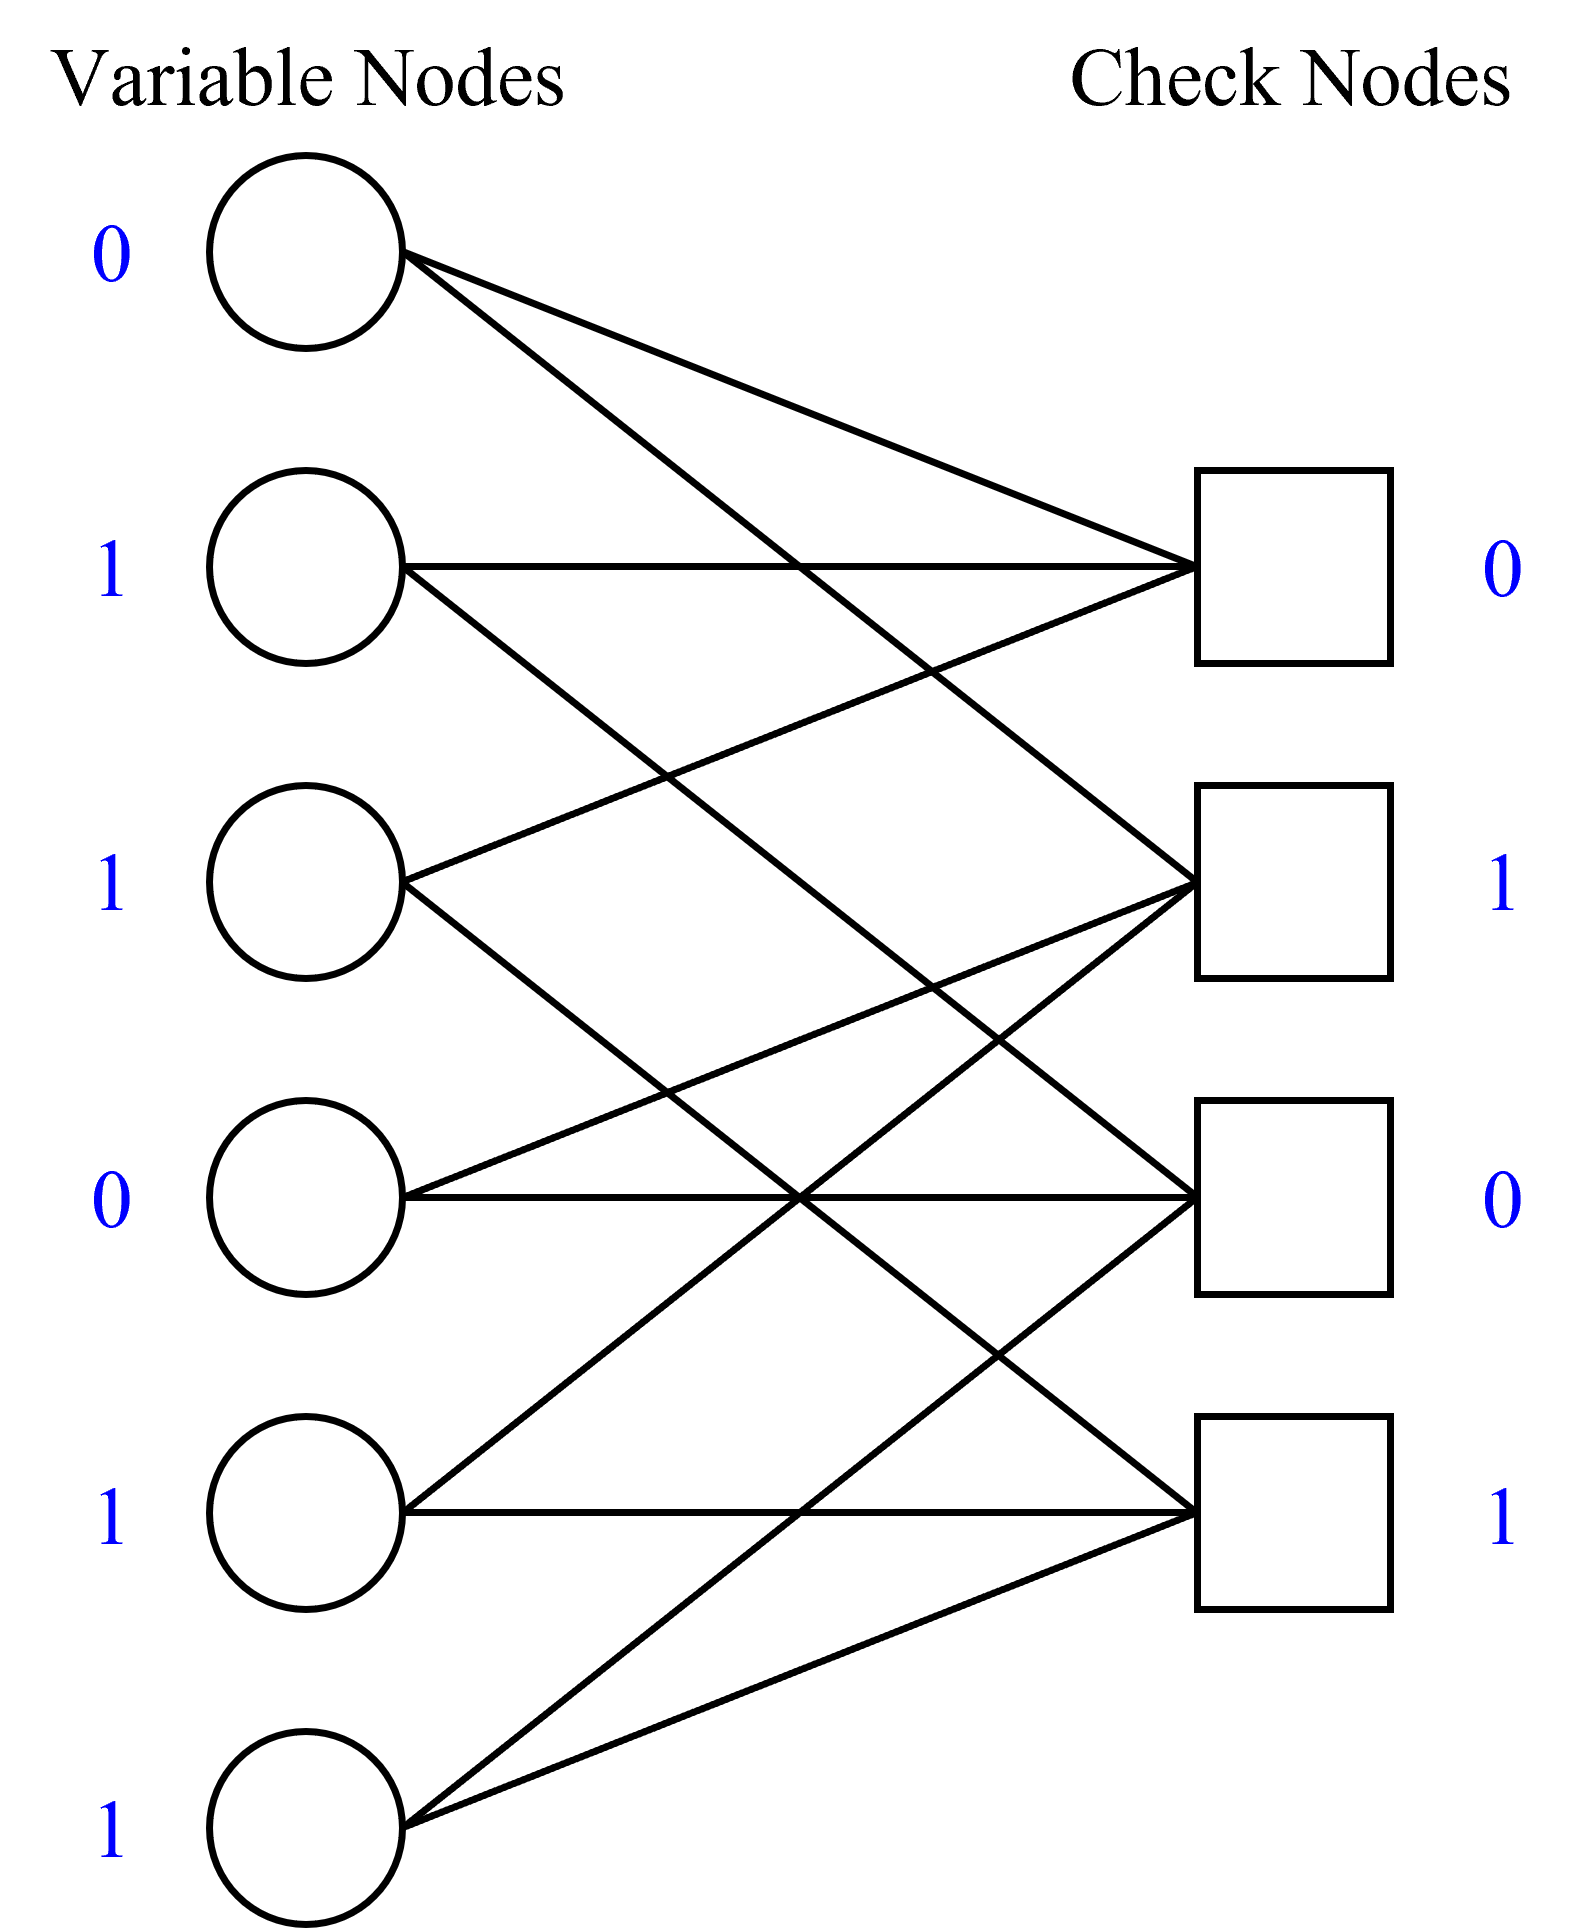
\includegraphics[width=0.4\linewidth]{figures/w10_LDPC.png}
    \caption{Tanner graph of an LDPC code.}
    \label{fig:w10_LDPC}
\end{figure}

The graph consists of two types of nodes: variable nodes (VN) which carry information, and check nodes (CN) who's check sums determine the symptom of a received word. A valid codeword is equal to a vector of assignments on the variable nodes such that all values to the check nodes are zero, else the word is corrupted.

To draw a Tanner graph, it is required that the VN's are drawn on the left, indicated by circular nodes, and the CN's are drawn on the right, indicated by square nodes. Besides \autoref{fig:w10_LDPC}, the only allowed variant of drawing a Tanner graph is \autoref{fig:w10_LDPC_horizontal}.

\begin{figure}[H]
    \centering
    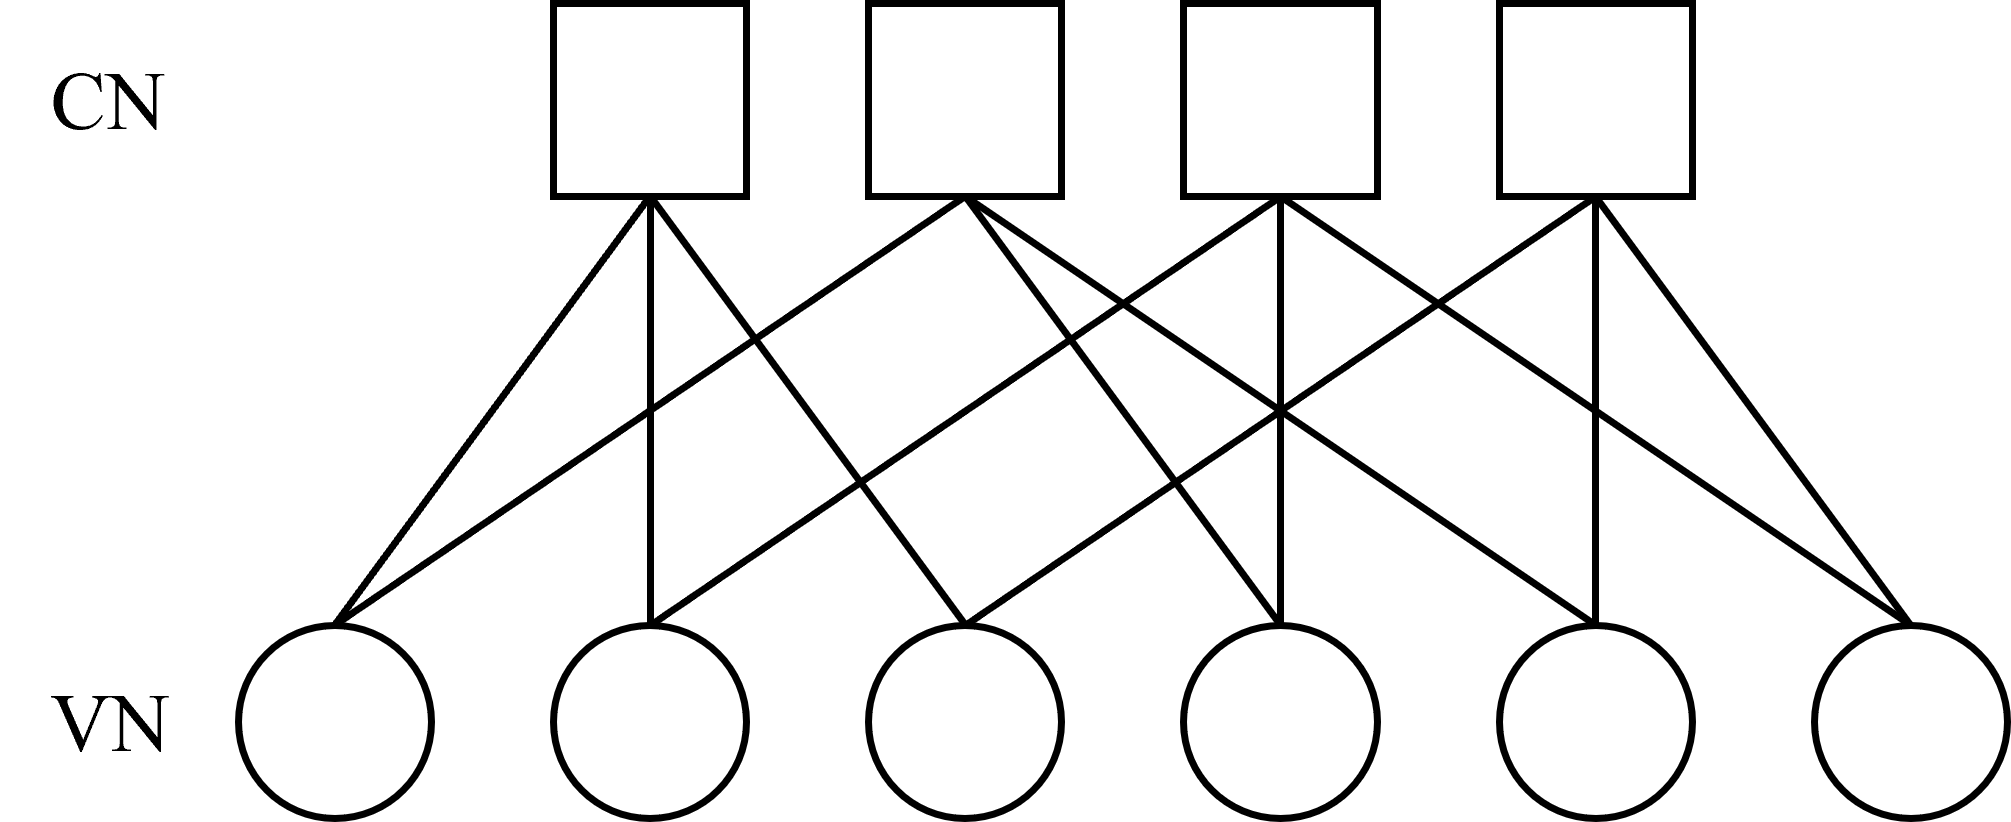
\includegraphics[width=0.5\linewidth]{figures/w10_LDPC_horizontal.png}
    \caption{Horizontal Tanner graph.}
    \label{fig:w10_LDPC_horizontal}
\end{figure}

\begin{definition}[Parity-Check Matrix Formulation]
    An LDPC code can be uniquely defined by the \textit{biadjacency matrix} $H\in\mathbb{F}_2^{\abs{\mathrm{VN}}\times\abs{\mathrm{CN}}}$ of the bipartite graph, where $\mathrm{VN}$ is the set of variable notes, and $\mathrm{CN}$ is the set of check nodes. The graph is also called a \textit{Tanner graph}.

    The biadjacency matrix is related to the \textit{adjacency matrix} of the Tanner graph by
    \begin{equation}
        A = \left[\begin{matrix}
            0 & H \\ H^\transpose & 0
        \end{matrix}\right],
    \end{equation}
    where the first $\abs{\mathrm{VN}}$ rows and columns are the VN's, and the latter $\abs{\mathrm{CN}}$ rows and columns are the CN's.
\end{definition}

\begin{example}
    Take \autoref{fig:w10_LDPC} as an example. Listing the ten vertices in order from VN to CN, from top to bottom, we have the following biadjacency matrix:
    \begin{equation*}
        H = \left[\begin{matrix}
            1 & 1 & 0 & 0 \\
            1 & 0 & 1 & 0 \\
            1 & 0 & 0 & 1 \\
            0 & 1 & 1 & 0 \\
            0 & 1 & 0 & 1 \\
            0 & 0 & 1 & 1 
        \end{matrix}\right].
    \end{equation*}
    Given a word $w\in\mathbb{F}_2^{\abs{\mathrm{VN}}\times 1}$, one can check whether it is a valid codeword by seeing if $Hw$ is the zero vector or not.
\end{example}

\begin{theorem}[Rate of LDPC Code]
    The rate $R$ of an LDPC code satisfies
    \begin{equation}
        R \ge 1- \frac{\abs{\mathrm{CN}}}{\abs{\mathrm{VN}}},
    \end{equation}
    where the equality is met if and only if $H$ is full rank.
\end{theorem}



\section{LDPC over BEC}
Below we see a couple of examples of LDPC over BEC,

\begin{figure}
    \centering
    \subfloat[Single parity-check code.]{
        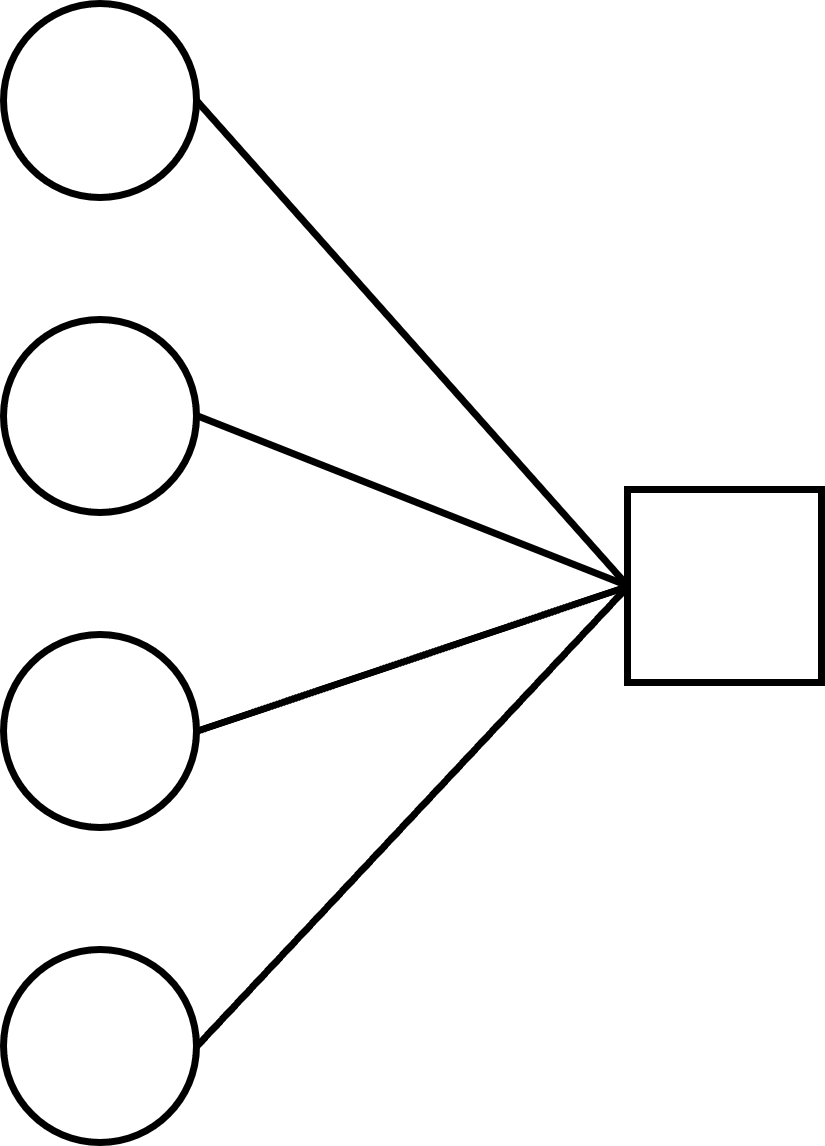
\includegraphics[width=0.25\textwidth]{figures/w10_SPC.png}
        \label{fig:w10_SPC}
    }
    \hspace{1cm}
    \subfloat[Repetition code.]{
        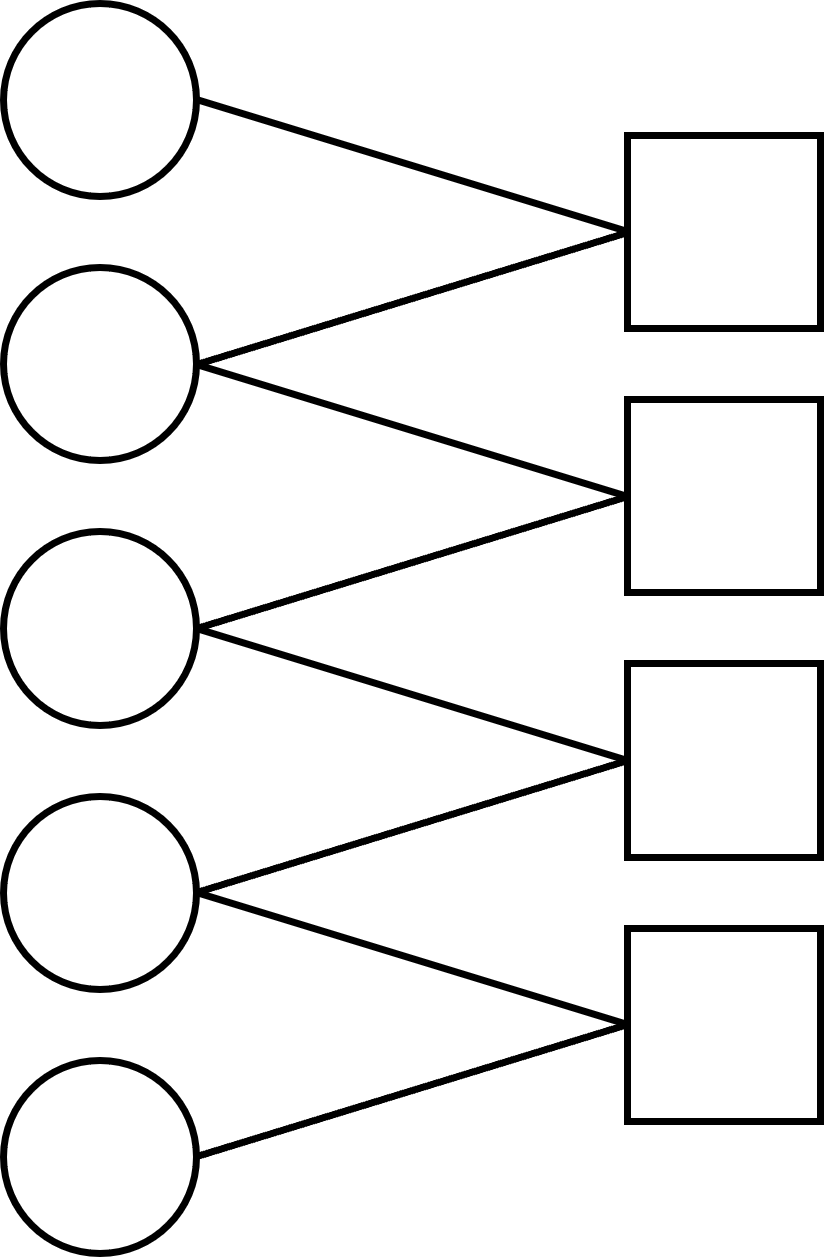
\includegraphics[width=0.25\textwidth]{figures/w10_RC.png}
        \label{fig:w10_RC}
    }
    \hspace{1cm}
    \subfloat[Onion-peeling decoding.]{
        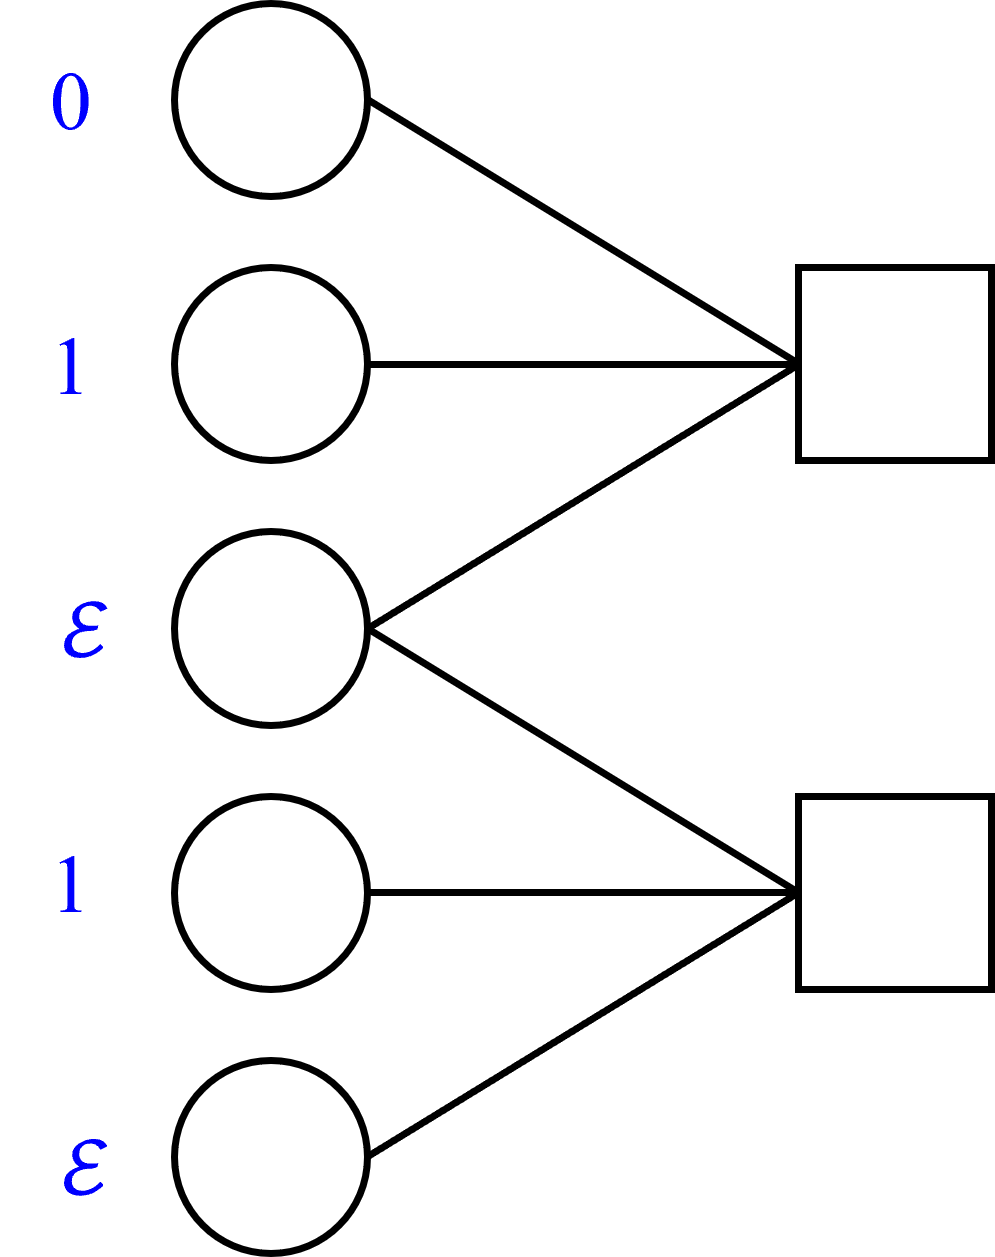
\includegraphics[width=0.28\textwidth]{figures/w10_onion.png}
        \label{fig:w10_onion}
    }
    \caption{LDPC over BEC}
\end{figure}

\begin{example}
    \autoref{fig:w10_SPC} shows the Tanner graph of a single parity-check (SPC) code. The biadjacency matrix of the code is the matrix of ones $H = [1,1,1,1]^\transpose$. If one receives a codeword with a single erasure, say $[0,1,0,\mathcal{E}]^\transpose$, it can be readily seen from the check sum that the erasure should be a 1. However, if there are more than one erasures, say $[0,\mathcal{E},0,\mathcal{E}]^\transpose$, nothing can be learned. Hence, we see that SPC can deal with code having only one erasure.
\end{example}

\begin{example}
    \autoref{fig:w10_RC} shows the Tanner graph of a repetition code (RC). Its biadjacency matrix is a \textit{Toeplitz matrix} of the form
    \begin{equation*}
        H = \left[\begin{matrix}
            1 \\
            1 & 1 \\
            & 1 & 1 \\
            & & 1 & 1 \\
            & & & 1
        \end{matrix}\right],
    \end{equation*}
    and the generator matrix of the codebook is $G=[1,1,1,1,1]$.
\end{example}

\begin{example}
    In \autoref{fig:w10_onion}, we consider decoding with a not-so-trivial LDPC code over a BEC channel. Upon receiving $[0,1,\mathcal{E},0,\mathcal{E}]$, the first CN can immediately recognize that the first erasure is 1. After finding out the first erasure, the second erasure can be determined to be 0 from the second CN.

    This decoding method is called the ``\textit{onion-peeling decoder}.'' Other names exist, too, including the iterative decoder, and my favorite -- the ``sudoku decoder.''
\end{example}

\begin{definition}[Stopping Set / Trapping Set]
    A subset of VN that cannot be decoded if they are all erasure is called a stopping set.
\end{definition}
A stopping set can be removed by adding a new check node, connecting to variable nodes both in the stopping set and outside of the stopping set. However, this decreases the code rate.

\begin{example}
    A common example of stopping sets are cycles. \autoref{fig:w10_cycles} are some examples.
    \begin{figure}[H]
        \centering
        \subfloat[4-cycle.]{
            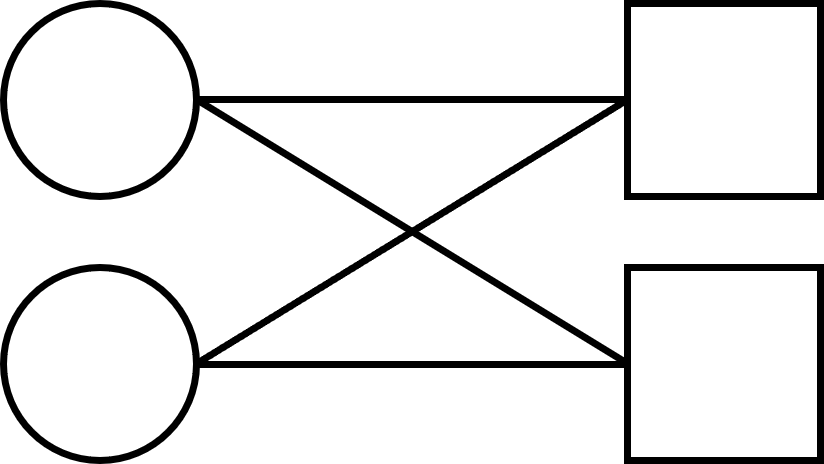
\includegraphics[width=0.2\textwidth]{figures/w10_4cycle.png}
        }
        \hspace{1cm}
        \subfloat[6-cycle.]{
            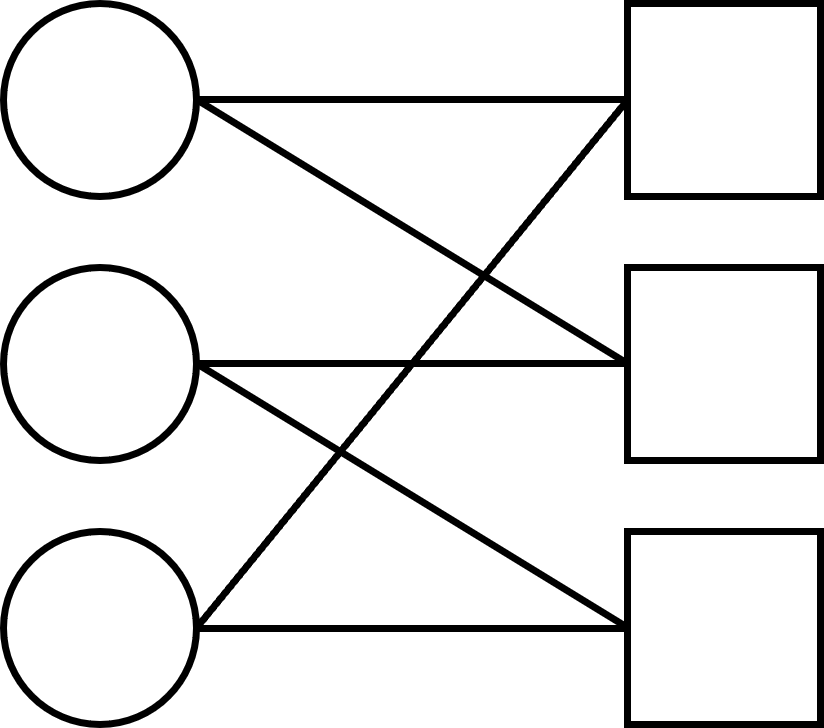
\includegraphics[width=0.2\textwidth]{figures/w10_6cycle.png}
        }
        \caption{Cycles as trapping sets.}
        \label{fig:w10_cycles}
    \end{figure}
    Let the block length of the code be $N$, which is often in the orders of thousands, finding a 4-cycle requires traversing the graph by brute force, requiring a complexity of $O(N^4)$. Similarly, for 6-cycles, $O(N^6)$ computations are needed. The complexity quickly go out of control as the size of the cycle one wish to check increases.
\end{example}


\subsection{Decoding Analysis}
To see whether a setup of VN's and CN's can be decoded, we can analyze the performance on a random graph instead.

\begin{definition}[Regular Graph]
    A graph is regular if $\deg v$ is a constant for all vertex $v$, where $\deg v$ is the amount of edges the vertex is connected to.
\end{definition}

\begin{definition}[Regular LDPC]
    An LDPC code is regular if the degree of the VN's (variable degree) and the degree of the CN's (check degree) are constants.
\end{definition}

\begin{example}
    A $[3,6]$-LDPC is one where its variable degree is 3, and its check degree is 6.
\end{example}

Here we will be dealing with regular LDPC codes, especially having the degree of VN's be 3 and the degree of CN's be 6 such that the rate is $R=1/2$.

Pick a random graph that satisfies the above setup and send a codeword over $\mathrm{BEC}(x)$. Initially, the fraction of VN's that remain as erasures is $x_0\defeq x$.
\begin{figure}[H]
    \centering
    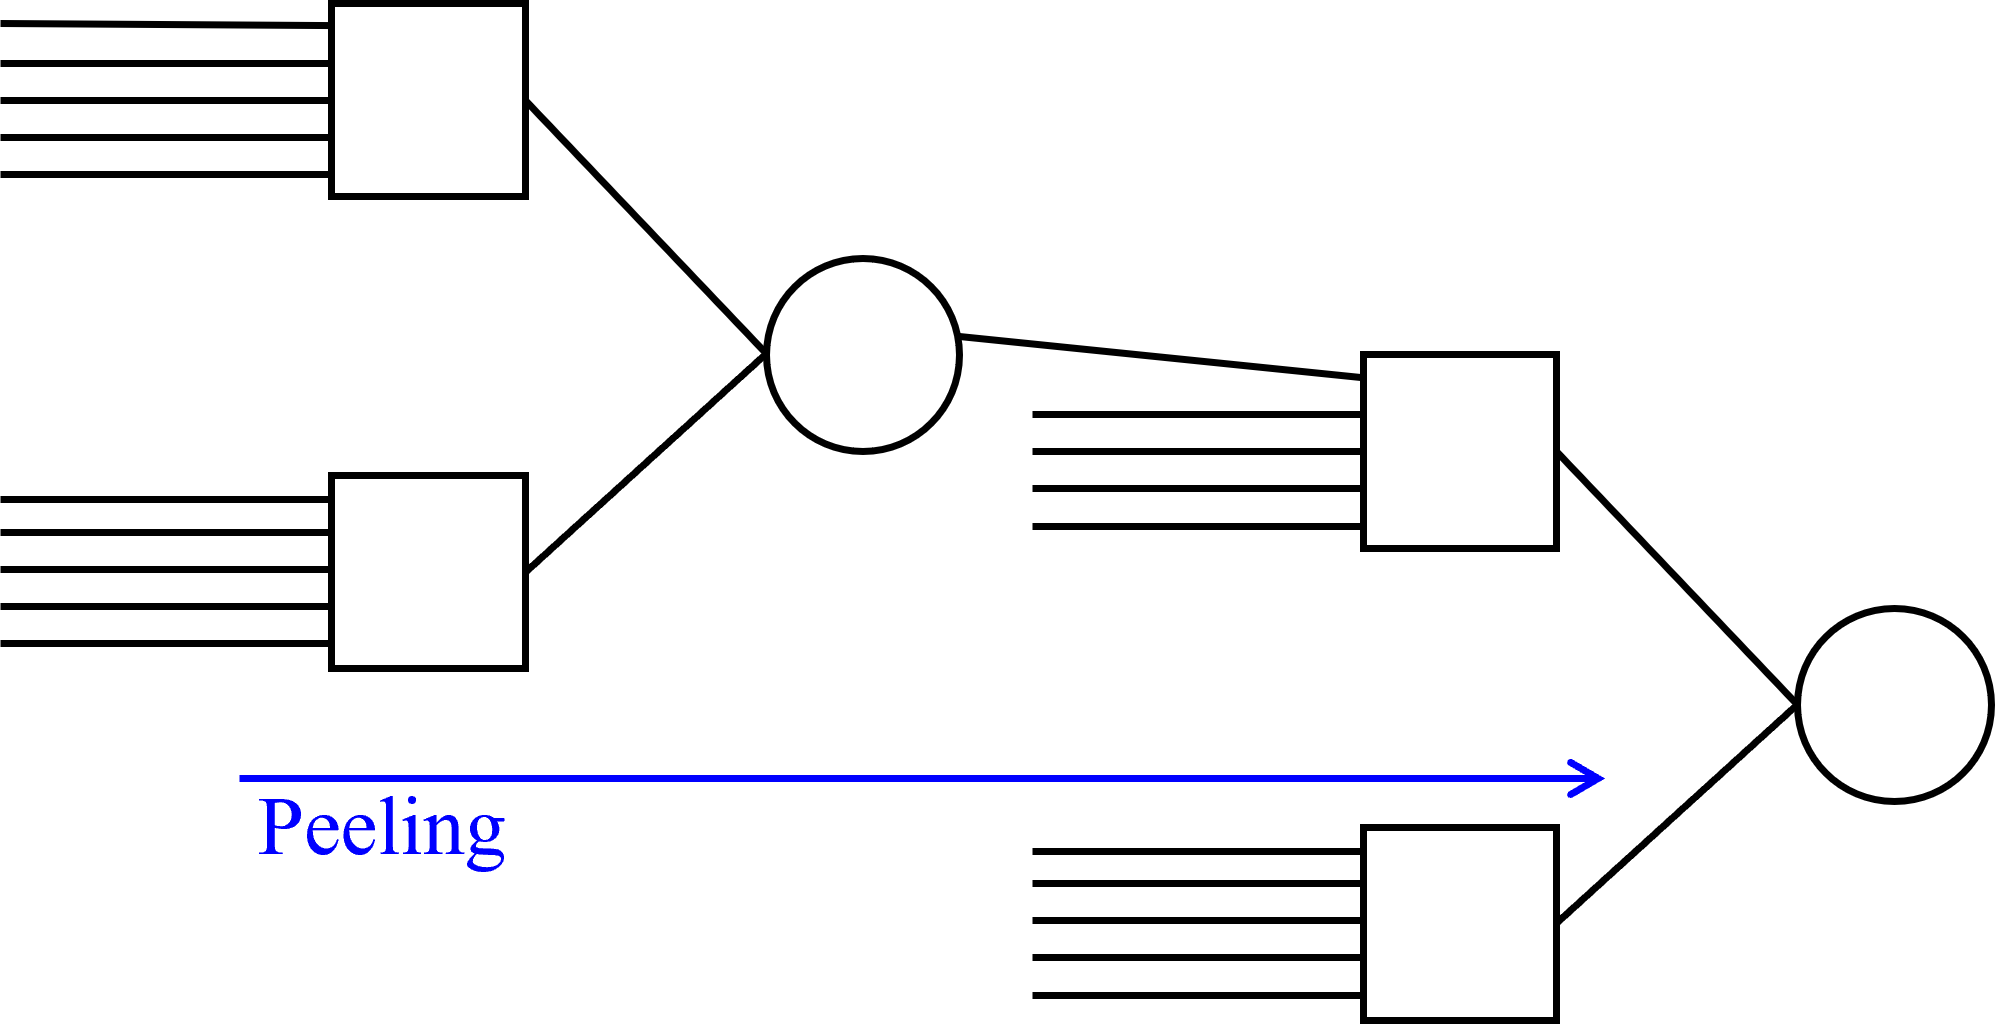
\includegraphics[width=0.5\linewidth]{figures/w10_decoding.png}
    \caption{Tree of onion-peeling / sudoku decoding.}
    \label{fig:w10_decoding}
\end{figure}
After a layer of onion-peeling decoding, a VN that was originally an erasure (say the first VN drawn in \autoref{fig:w10_decoding}) can be decoded if at least one of the check nodes on its left connects to no other erasures. I.e., the remaining fraction of erasures after an iteration becomes
\begin{equation*}
    x_1 \defeq x \left(1-(1-x)^5\right)^2
\end{equation*}
on expectation. If we peel again, the remaining fraction of erasures become
\begin{equation*}
    x_2 \defeq x\left(1-(1-x_1)^5\right)^2.
\end{equation*}
And we do this again and again until achieving $x_n\rightarrow0$, then we ``believe'' that this code is good enough.

Though the iteration is strictly decreasing, it does not always converge to zero. See \autoref{fig:w10_iter_conv} below. Let us consider the code having a rate $R=1/2$, what parameters can the $x_0$ in $\mathrm{BEC}(x_0)$ be so that codewords can be successfully decoded? In theory, the optimal case is $x_0=1/2$. However, by drawing out the iteration
\begin{equation}
    x_n = x_0 \left(1-(1-x_{n-1})^5\right)^2 \label{eq:w10_iteration_example}
\end{equation}
via \autoref{fig:w10_iter_conv_1}, we can see that only when $x_0\lesssim 0.42944$ will the sequence converge to zero. Hence, LDPC code is NOT capacity-achieving.

\begin{figure}[H]
    \centering
    \subfloat[(Part of a) Cobweb plot.]{
        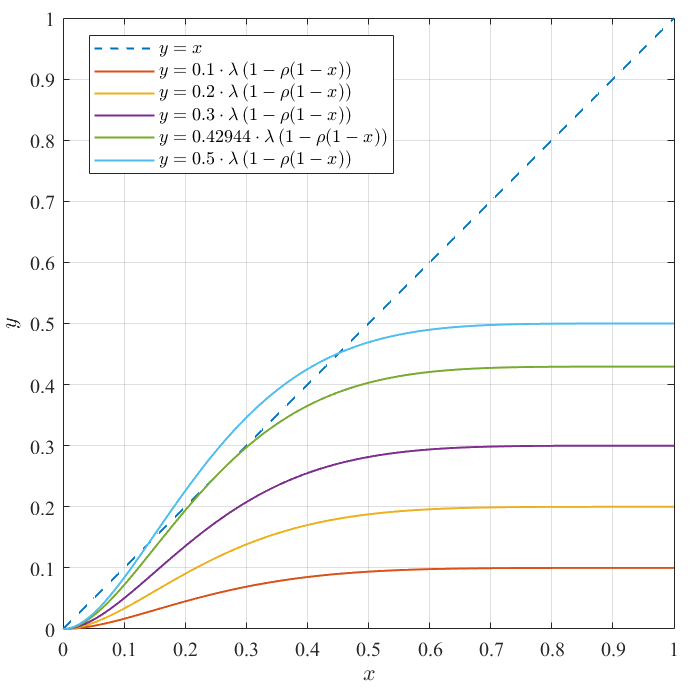
\includegraphics[width=0.475\linewidth]{figures/w10_iter_conv.png}
        \label{fig:w10_iter_conv_1}
    }
    \hspace{0.1cm}
    \subfloat[EXIT chart.]{
        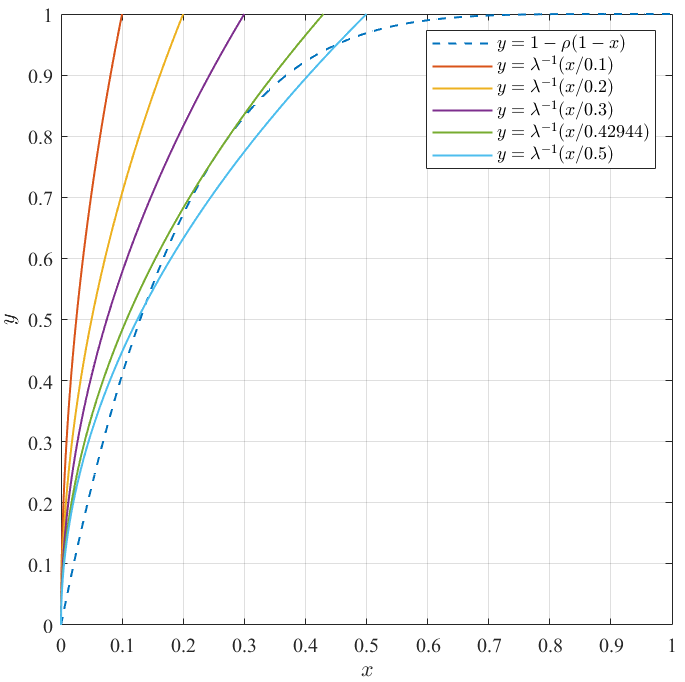
\includegraphics[width=0.475\textwidth]{figures/w10_EXIT_chart.png}
        \label{fig:w10_iter_conv_EXIT}
    }
    \caption{Convergence of fraction of erasures through decoding.}
    \label{fig:w10_iter_conv}
\end{figure}

Another often seen diagram of showing the convergence of the fraction of erasures is the EXIT graph, as seen in \autoref{fig:w10_iter_conv_EXIT}. It performs a transformation on the two curves $y=x$ and $y=x_0(1-(1-x)^5)^2$ to make the analysis for more complicated Tanner graphs simpler, as we will see in the next section.

\section{Irregular LDPC}
In this section we discuss a general LDPC code, containing nodes of various degrees not constrained to be constants, called irregular LDPC.

\begin{definition}[Irregular LDPC]
    For an irregular LDPC, various terms can be defined:
    \begin{itemize}
        \item From the perspective of nodes:
        \begin{align}
            \Lambda_i &\defeq \#\text{ of VN with degree } i, \\
            P_i &\defeq \#\text{ of CN with degree } i,
        \end{align}
        The generating function of the two enumerators are denoted as
        \begin{align}
            \Lambda(x) &\defeq \sum_{i} \Lambda_i x^i, \\
            P(x) &\defeq \sum_{i} P_i x^i.
        \end{align}
        $\Lambda$ and $P$ are the \textit{variable} and $\textit{check degree distributions from a node perspective}$. The normalized degree distributions are
        \begin{align}
            L_i &\defeq \frac{\#\text{ of VN of degree } i}{\#\text{VN}} = \frac{\Lambda_i}{\Lambda(1)}, &L(x) \defeq \sum_{i} L_i x^i = \frac{\Lambda(x)}{\Lambda(1)}, \\
            R_i &\defeq \frac{\#\text{ of CN of degree } i}{\#\text{CN}} = \frac{P_i}{P(1)}, &R(x) \defeq \sum_{i} R_i x^i = \frac{P(x)}{P(1)},
        \end{align}
        the letter $L$ and $R$ stands for left and right, respectively.
        \item From the perspective of edges:
        \begin{align}
            \lambda(x) = \sum_{i} \lambda_i x^{i-1} &\defeq \frac{\Lambda'(x)}{\Lambda'(1)} = \frac{L'(x)}{L'(1)}, \\
            \rho(x) = \sum_{i} \rho x^{i-1} &\defeq \frac{P'(x)}{P'(1)} = \frac{R'(x)}{R'(1)}.
        \end{align}
        The coefficient $\lambda_i\propto i\Lambda_i$ (resp. $\rho_i\propto iP_i$) equals to the fractions of edges that connect to VN's (resp. CN's) of degree $i$. We call $\lambda$ and $\rho$ are the \textit{variable} and \textit{check degree distributions from an edge perspective}.
    \end{itemize}
\end{definition}

\begin{example}
    For a regular LDPC, say the $[3,6]$-LDPC, we have $L(x)=x^3$ and $R(x)=x^6$, with $\lambda(x)=x^2$ and $\rho(x)=x^5$. Note that the iteration \autoref{eq:w10_iteration_example} can be rewritten as
    \begin{equation}
        x_{n} = x_0 \cdot \lambda\left(1-\rho(1-x)\right).
    \end{equation}
    This result can be further generalized.
\end{example}

Consider $L(x) = \frac{1}{2}x^3 + \frac{1}{2}x^4$ and $R(x) = \frac{2}{3}x^6 + \frac{1}{3}x^{20}$. We have $\lambda(x) = \frac{3}{7}x^2 + \frac{4}{7}x^3$ and $\rho(x) = \frac{3}{8}x^5 + \frac{5}{8}x^{19}$. Its Tanner graph can be roughly drawn as in \autoref{fig:w10_irregular_LDPC}, it is a random ensemble of LDPC codes.

\begin{figure}[h]
    \centering
    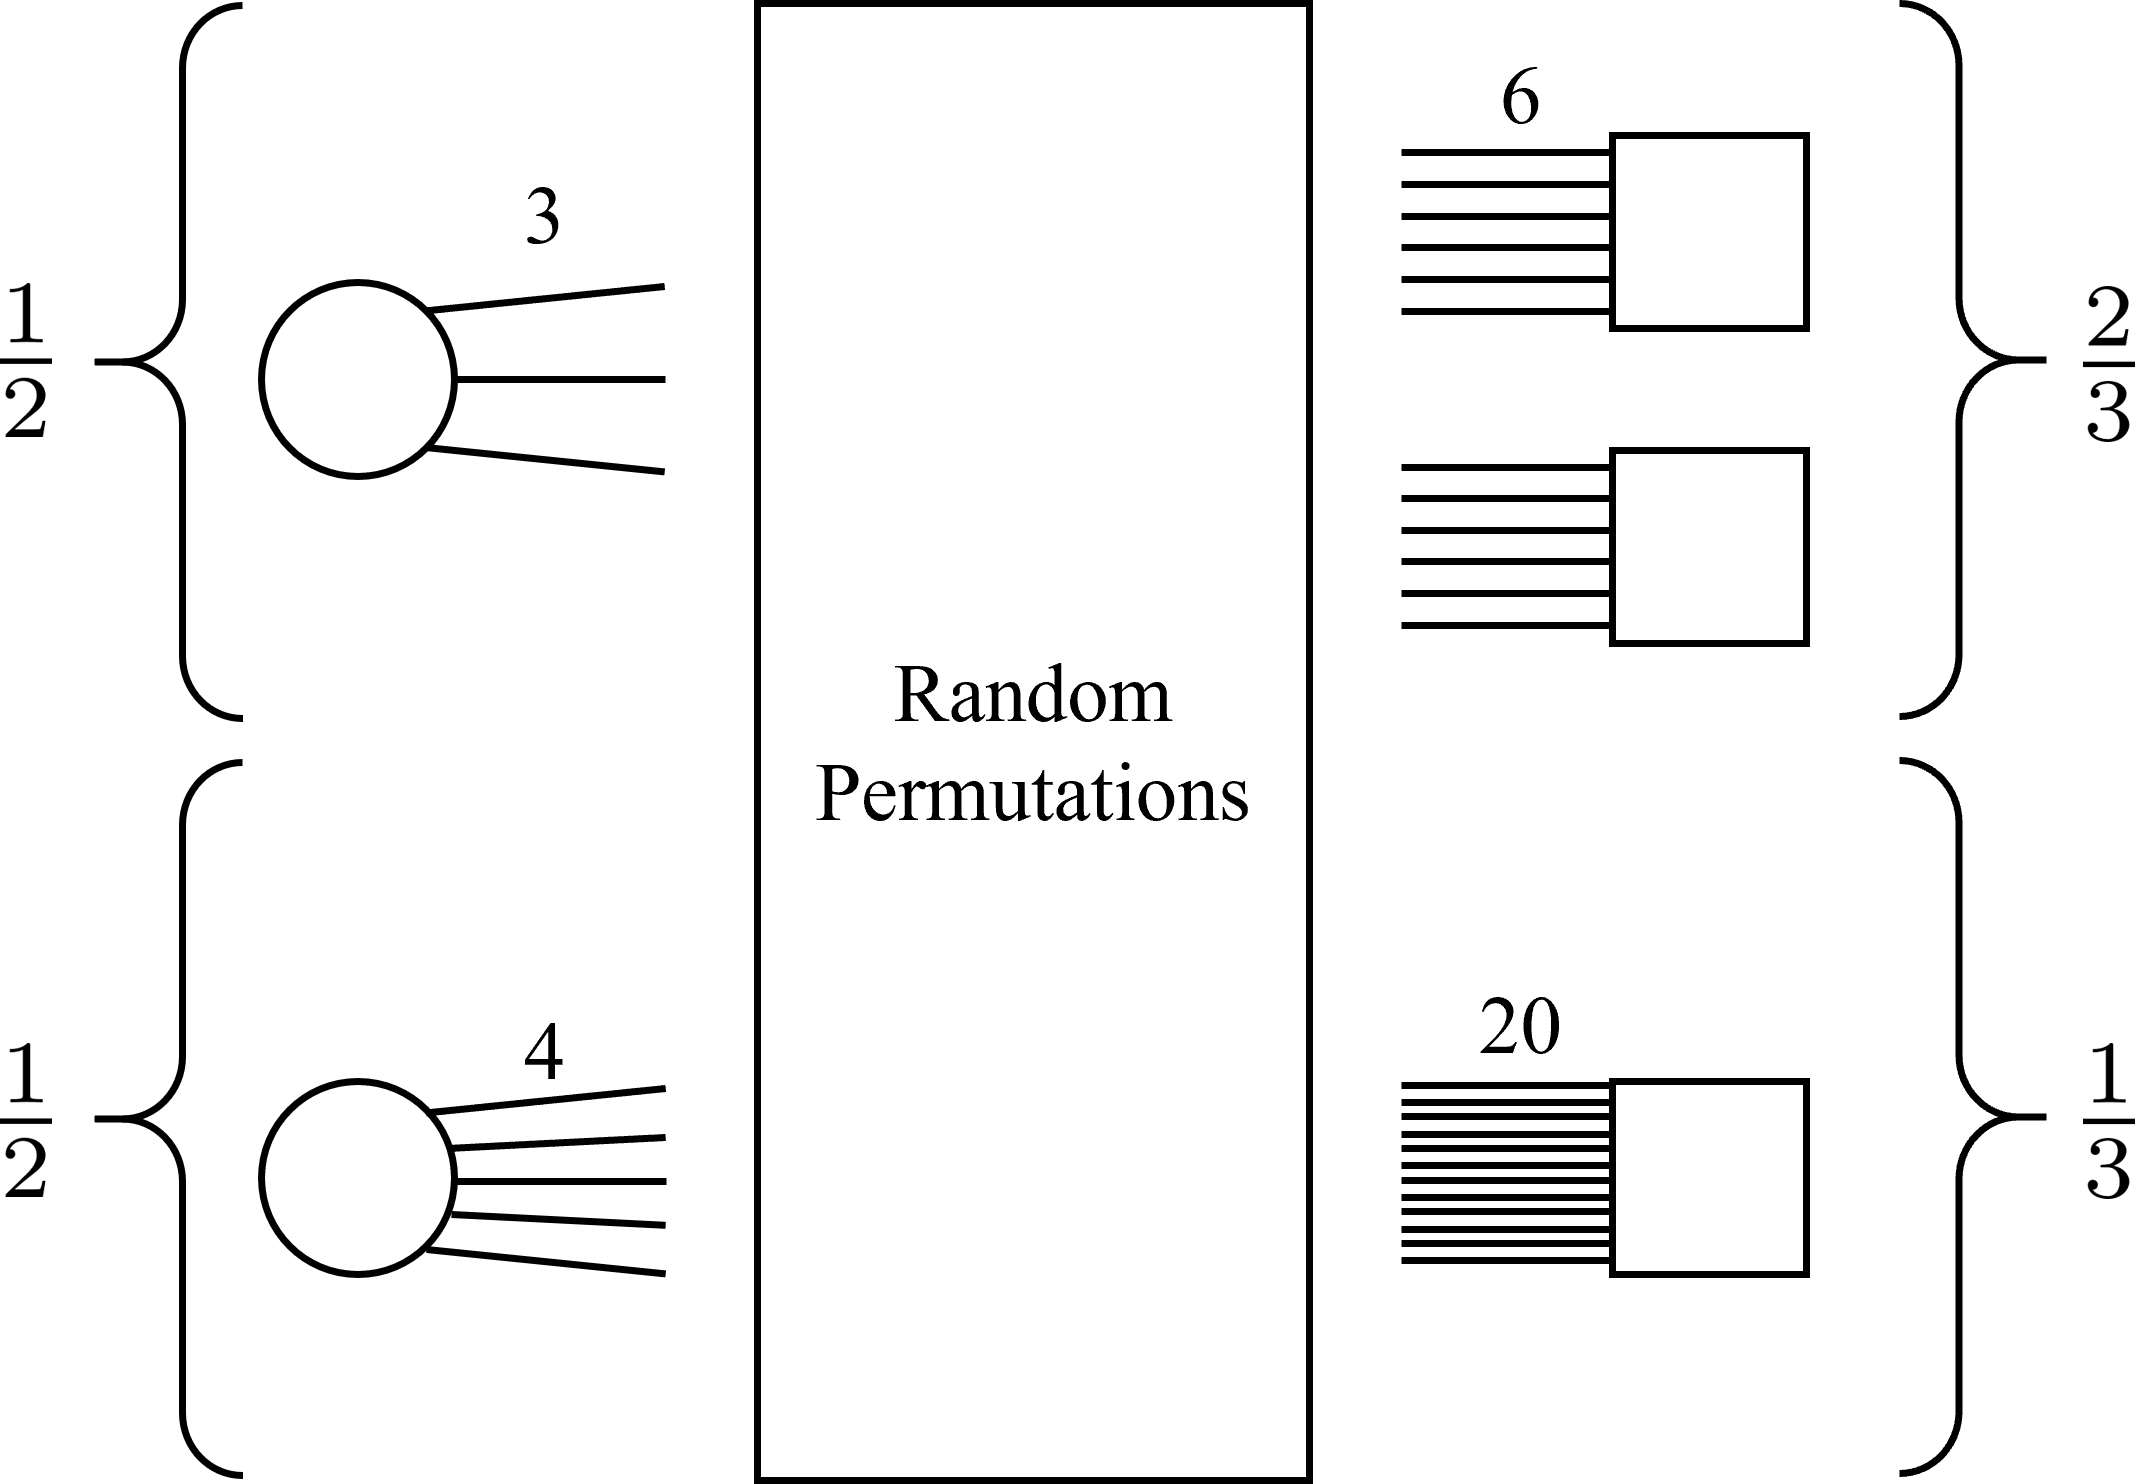
\includegraphics[width=0.5\linewidth]{figures/w10_irregular_LDPC.png}
    \caption{Irregular LDPC with $L(x) = \frac{1}{2}x^3 + \frac{1}{2}x^4$ and $R(x) = \frac{2}{3}x^6 + \frac{1}{3}x^{20}$.}
    \label{fig:w10_irregular_LDPC}
\end{figure}

When applying onion-peeling decoding (refer to \autoref{fig:w10_decoding}), a VN (say $\mathrm{VN}_1$) connects to CN's with 6 edges with probability $\rho_6$, and CN's with 20 edges with probability $\rho_{20}$. Of these CN's with 6 or 20 edges, only 5 or 19 edges are connected to the other VN's. If $\mathrm{VN}_1$ can be decoded successfully, it requires that at least one of the CN's that it is connected to connects to no other erasures. Suppose the fraction of erasures is $x$, the probability on average for a single CN to connect to no erasure is
\begin{equation*}
    \frac{3}{8}(1-x)^5 + \frac{5}{8}(1-x)^{19} = \rho_6(1-x)^5 + \rho_{20}(1-x)^{19} = \rho(1-x).
\end{equation*}
And for each CN, it connects to a degree 3 $\mathrm{VN}_1$ with probability $\lambda_3$, and to a degree 4 $\mathrm{VN}_1$ with probability $\lambda_4$. Since one extra edge of $\mathrm{VN}_1$ should be used to help the future decoding, if $\mathrm{VN}_1$ has degree $i$, we only need one of the remaining $i-1$ check nodes it connected to be helpful. The probability on average that none of the CN's it is connected to is helpful in its decoding will be
\begin{equation*}
    \frac{3}{7}(1-\rho(1-x))^2 + \frac{4}{7}(1-\rho(1-x))^3 = \lambda_3(1-\rho(1-x))^2 + \lambda_4(1-\rho(1-x))^3 = \lambda(1-\rho(1-x)).
\end{equation*}
Henceforth, we see:
\begin{theorem}[Density Evolution] \label{thm:w10_density_evolution}
    The evolution of the density of erasures of an LDPC over $\mathrm{BEC}(x_0)$ after $n$ iterations of decoding follows the following iteration:
    \begin{equation}
        x_{n} = x_0 \cdot \lambda(1-\rho(1-x_{n-1})).
    \end{equation}
\end{theorem}

The iteration between the functions
\begin{align*}
    y_{n} &= x_0\cdot\lambda(1-\rho(1-x_{n-1})),\\
    x_{n} &= y_n
\end{align*}
can be translated the iteration between the functions
\begin{align*}
    y_{n} &= 1 - \rho(1-x_{n-1}), \\
    x_n &= x_0\lambda(y_{n}).
\end{align*}
We can again draw the cobweb plot and EXIT chart as \autoref{fig:w10_iter_conv_2} below. 

The design of a suitable code will hence be translated to the design of suitable polynomials $\rho$ and $\lambda$.

\begin{figure}[H]
    \centering
    \subfloat[Cobweb plot.]{
        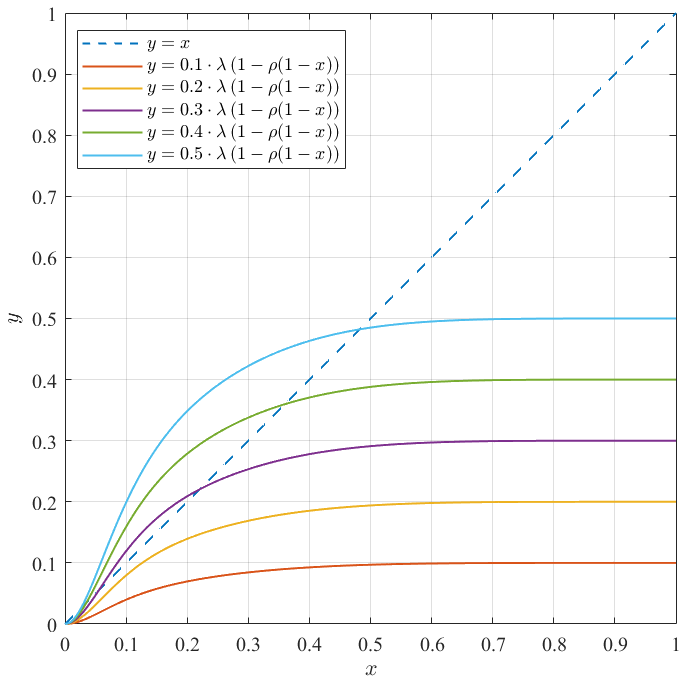
\includegraphics[width=0.475\textwidth]{figures/w10_iter_conv_2.png}
    }
    \hspace{0.1cm}
    \subfloat[EXIT chart.]{
        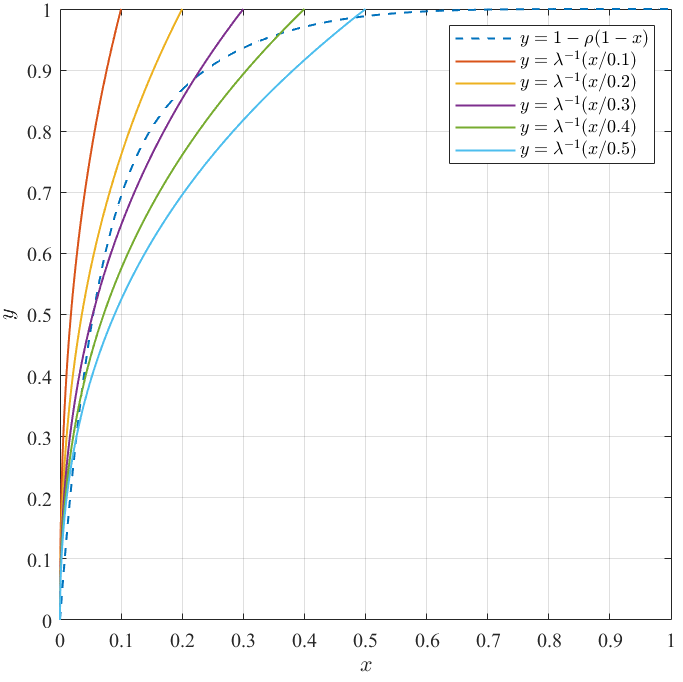
\includegraphics[width=0.475\textwidth]{figures/w10_EXIT_chart_2.png}
    }
    \caption{Convergence of fraction of erasures for $\lambda(x) = \frac{3}{7}x^2 + \frac{4}{7}x^3$ and $\rho(x) = \frac{3}{8}x^5 + \frac{5}{8}x^{19}$.}
    \label{fig:w10_iter_conv_2}
\end{figure}
